\documentclass[11pt,a4paper]{ctexart}

\usepackage[margin=2.2cm]{geometry}
\usepackage{amsmath,amssymb,amsthm,mathtools}
\usepackage[dvipsnames]{xcolor}
\usepackage{hyperref}
\usepackage{enumitem}
\usepackage[most]{tcolorbox}
\usepackage{tikz}
\usetikzlibrary{arrows.meta,decorations.pathmorphing}

\hypersetup{colorlinks=true,linkcolor=blue!55!black,urlcolor=blue!55!black}
\setlist[enumerate]{itemsep=0.35em,topsep=0.45em}
\setlist[itemize]{itemsep=0.35em,topsep=0.45em}

\newtheorem{principle}{朴素原理}[section]
\newtheorem{example}[principle]{生活例子}

\tcbset{
  commonbox/.style={enhanced,breakable,boxrule=0.8pt,arc=2mm,
    left=1.4mm,right=1.4mm,top=1mm,bottom=1mm,colback=white}
}
\newtcolorbox{newsblock}{commonbox,colframe=BrickRed!65!black,colback=BrickRed!4,
  title=新闻里说了什么,fonttitle=\bfseries}
\newtcolorbox{intuitionblock}{commonbox,colframe=RoyalBlue!70!black,colback=RoyalBlue!4,
  title=朴素直觉,fonttitle=\bfseries}
\newtcolorbox{lifeblock}{commonbox,colframe=ForestGreen!60!black,colback=ForestGreen!4,
  title=生活类比,fonttitle=\bfseries}
\newtcolorbox{keypointblock}{commonbox,colframe=black!65,colback=black!3,
  title=一句话记住,fonttitle=\bfseries}
\newtcolorbox{mathblock}[1]{commonbox,colframe=Purple!60!black,colback=Purple!4,
  title=#1,fonttitle=\bfseries}

\title{从一则量子新闻里能挖出哪些朴素物理\\
  \large 解读：``原子钟技术验证时间存在量子叠加态''}
\author{}
\date{\today}

\begin{document}
\maketitle

\begin{newsblock}
2026 年 4 月 22 日新华社报道：美国史蒂文斯理工学院的研究者将单个铝/镱离子囚禁、
冷却到接近绝对零度，再用激光精确操控其量子态。他们的理论分析（发表于
《物理评论快报》）表明，把高精度原子钟和离子量子计算结合起来，原则上可以
让一台时钟同时``走得快''和``走得慢''——也就是\emph{时间流逝本身}处于量子
叠加态。这是 2010 年代提出的``量子孪生子佯谬''首次接近可观测。
\end{newsblock}

\tableofcontents
\newpage

\section{新闻里其实藏了几条物理}

这则报道字数不多，但同时用到了\textbf{相对论}、\textbf{量子力学}、
\textbf{原子钟原理}和\textbf{量子涨落}。我们不去做严格推导，只把每一条
拆成``一个朴素原理 + 一个生活例子''，让初学者也能记住。

下面 5 条原理就是这次能挖到的全部干货：

\begin{enumerate}[label=\textbf{原理\arabic*.}]
  \item 不同观察者的时钟走得不一样（相对论的``固有时间''）。
  \item 任何振荡稳定的东西都可以当时钟（原子钟为什么准）。
  \item 微观系统可以同时处于几个状态（量子叠加）。
  \item 把时钟也当成量子系统时，它的``读数''也能叠加（量子孪生子佯谬）。
  \item 真空不空，零度不静（量子涨落与压缩态）。
\end{enumerate}

\section{原理 1：每个时钟有自己的``固有时间''}

\begin{newsblock}
原文：``在相对论中，每一台时钟都拥有各自的固有时间，其流逝取决于速度和所处位置。''
\end{newsblock}

\begin{intuitionblock}
\textbf{朴素说法。}时间不是宇宙挂在墙上的一只大钟，而是\emph{每一只钟自己
身上的事}。你跑得越快，你的钟相对地面就走得越慢；你站得越低（引力越强），
你的钟也走得越慢。
\end{intuitionblock}

\begin{mathblock}{用一行公式}
对一个相对地面以速度 $v$ 运动的钟，
\[
  \Delta\tau \;=\; \Delta t\,\sqrt{1-\tfrac{v^{2}}{c^{2}}}
  \;\le\; \Delta t,
\]
$\Delta\tau$ 是运动钟自己读到的时间，$\Delta t$ 是地面钟读到的时间。
$v$ 越接近光速 $c$，根号越小，运动钟越``年轻''。
\end{mathblock}

\begin{example}[GPS 导航]
GPS 卫星距地约 2 万公里、绕地球高速运动。\emph{速度}让卫星钟变慢，
\emph{高引力位}让它变快，两者综合后卫星钟比地面快约 $38\,\mu s/$天。
如果不修正这 38 微秒，1 天后导航定位就会偏出大约 11 公里——
你的导航 App 之所以能告诉你``下一个路口右拐'', 背后真的在做相对论修正。
\end{example}

\begin{example}[爬楼梯也变``老'']
顶楼的钟比一楼的钟快得不到 $10^{-16}$，意味着你在 30 层办公一辈子，
比一楼同事老了大约一百亿分之一秒。听上去为零，但今天最好的原子钟已经
能直接测出这个差。
\end{example}

\section{原理 2：任何稳定振荡都可以当时钟}

\begin{newsblock}
原文：``囚禁离子是一种多功能平台 \dots 用于量子计算和超高精度计时。''
\end{newsblock}

\begin{intuitionblock}
\textbf{朴素说法。}时钟的本质就是``数振动''。每一次振动定义一段``滴答''。
振动越稳定、越快，钟就越准。原子钟之所以准，是因为它\emph{数的是一个原子
能级跃迁的频率}，而这个频率由量子力学锁死，全宇宙的同种原子都一模一样。
\end{intuitionblock}

\begin{mathblock}{时间的基本定义}
1 秒 = 铯-133 原子在两个超精细能级间跃迁辐射 $9\,192\,631\,770$ 次的时间。
即
\[
  1\text{ s}\;\equiv\; 9\,192\,631\,770\,T_{\text{Cs}}.
\]
\end{mathblock}

\begin{example}[家里的石英表]
石英表里有一小块石英晶体，被电压一击就以 32\,768~Hz 振动，电路每数到
$2^{15}$ 次就让秒针跳一格。原理跟原子钟一样，只是``振子''不同：
石英片不如原子稳定，所以一年差几十秒；铝离子钟一年差不到一秒的
$10^{-10}$。
\end{example}

\begin{example}[心率与音乐节拍]
跑步时数节奏，听音乐打拍子，本质上你都在拿一个``周期事件''当时钟。
心率不稳，所以你不会拿心跳来对火车时刻；节拍器靠机械摆稳定一些，
所以乐手用它练琴。``越稳定越能当钟''是一条贯穿生活的原理。
\end{example}

\section{原理 3：微观系统可以同时处于几个状态}

\begin{newsblock}
原文：``根据量子理论，时间的流逝本身可能处于量子叠加态，即同时以更快和
更慢的速率流动。''
\end{newsblock}

\begin{intuitionblock}
\textbf{朴素说法。}对硬币来说，扔出去之前已经``是正面或反面''，只是
你不知道。对一个量子比特（比如一颗冷却的离子）来说，测量\emph{之前}
它真的是``既正又反''——这不是知识不足，而是物理事实。
\end{intuitionblock}

\begin{mathblock}{叠加态的写法}
两个基本状态 $\lvert 0\rangle$、$\lvert 1\rangle$，叠加态写成
\[
  \lvert\psi\rangle \;=\; \alpha\,\lvert 0\rangle + \beta\,\lvert 1\rangle,
  \qquad |\alpha|^2 + |\beta|^2 = 1.
\]
$|\alpha|^2$ 是你测到 0 的概率，$|\beta|^2$ 是测到 1 的概率。
测量之前，没有``真实的那一面''。
\end{mathblock}

\begin{center}
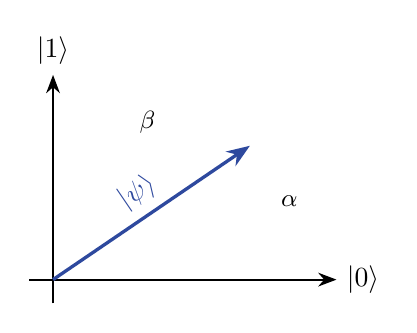
\begin{tikzpicture}[>=Stealth,scale=1.0]
  \draw[->,thick] (-0.3,0) -- (3.6,0) node[right]{$\lvert 0\rangle$};
  \draw[->,thick] (0,-0.3) -- (0,2.6) node[above]{$\lvert 1\rangle$};
  \draw[->,very thick,RoyalBlue!70!black] (0,0) -- (2.5,1.7)
        node[midway,above,sloped]{$\lvert\psi\rangle$};
  \node[font=\small] at (3.0,1.0) {$\alpha$};
  \node[font=\small] at (1.2,2.0) {$\beta$};
\end{tikzpicture}
\end{center}

\begin{example}[薛定谔的``导航路线'']
想象 App 给你两条路：A 路 30 分钟、B 路 32 分钟。在你点开之前，
经典世界里你``其实已经''走了某一条；如果是量子世界，你是\emph{两条
路都走了一点点}，到达终点时再被``测量''塌缩到其中一条。
现实生活里这不会发生，因为人和车太大；但对一个被囚禁的离子，
它走两条路是日常操作（双缝实验的现代版）。
\end{example}

\section{原理 4：让时钟自己叠加——量子孪生子佯谬}

\begin{newsblock}
原文：``一台时钟能否在量子叠加态中同时经历两种不同的时间流逝，从而
更年轻又更年老？''
\end{newsblock}

\begin{intuitionblock}
\textbf{朴素说法。}原理 1 告诉我们：钟跑得快慢不同，老化速度不同。
原理 3 告诉我们：微观系统可以同时处于多个状态。把两条放在一起就是
本次新闻的核心：让一台\emph{原子钟本身}同时处于两种运动状态，那么
它就会同时累积两份不同的``固有时间''——既更年轻又更年老。
\end{intuitionblock}

\begin{mathblock}{把时钟也写成叠加}
设``静止''与``高速''两条轨迹分别对应固有时间 $\tau_{\text{慢}}$、
$\tau_{\text{快}}$，原子内部状态记作 $\lvert\phi(\tau)\rangle$，则整体波函数大致为
\[
  \lvert\Psi\rangle \;=\;
  \tfrac{1}{\sqrt{2}}\Big(
    \lvert\text{慢}\rangle\otimes\lvert\phi(\tau_{\text{慢}})\rangle
    \;+\;
    \lvert\text{快}\rangle\otimes\lvert\phi(\tau_{\text{快}})\rangle
  \Big).
\]
位置自由度和``内部钟读数''纠缠在一起。这就是``量子孪生子''：
不需要两个孪生兄弟，一个钟自己就同时处在两种年龄。
\end{mathblock}

\begin{example}[``两条上班路'' 思想实验]
经典版：你和孪生兄弟，一个坐高铁出差一周，一个待在家。回来后高铁那位
\emph{年轻}了几纳秒。
量子版（实验室里）：你把\emph{自己一个人}放进叠加态，让你的``身体''
同时坐高铁又待在家。一周后做个干涉测量，会看到两个``你''重叠时
干涉条纹的相位里写着两份固有时间的差。
日常生活当然不会发生，但在被囚禁的冷离子上，``走两条路''就是这一类操作。
\end{example}

\section{原理 5：真空不空，零度不静}

\begin{newsblock}
原文：``即便在绝对零度条件下，量子涨落仍会影响时钟的计时速率 \dots
通过构造压缩态，直接调控量子真空，可使时钟的位置与速度呈现特殊的
量子关联。''
\end{newsblock}

\begin{intuitionblock}
\textbf{朴素说法。}经典物理里，温度降到 $0$ K 一切应该静止；
但量子力学告诉你，位置和动量不能同时为零，这就是
海森堡不确定性原理。所以哪怕冷到底，粒子还在抖，真空里也一直有``量子
噪声''。这点抖动会反过来影响时钟的频率读数。
\end{intuitionblock}

\begin{mathblock}{不确定性原理}
\[
  \Delta x \cdot \Delta p \;\ge\; \frac{\hbar}{2}.
\]
$\Delta x$ 是位置的不确定度，$\Delta p$ 是动量的不确定度，$\hbar$ 是
约化普朗克常数。两者一起逼近 $\hbar/2$ 的状态叫\textbf{压缩态}：
牺牲一个的精度去换另一个的精度。原子钟正是利用压缩态，把``时间噪声''
压低，从而\emph{看见}更细的相对论效应。
\end{mathblock}

\begin{example}[相机的 ISO 与快门]
拍夜景时，光子数有限，照片本身有``噪点''。提高 ISO 看得更亮，但噪点更多；
开大光圈进光多了，景深又变浅——你只能在两个``不确定度''之间分配预算。
这正是``压缩''的日常版：不是消除噪声，而是把噪声从你最在意的那一边挤
到不那么重要的另一边。
\end{example}

\begin{example}[听音叉对音]
两根音叉频率略有差别时会出``拍''——音量周期性强弱。原子钟的``叠加版本''
其实也在听拍：让原子内部能级相干叠加一段时间，再合并干涉，相位差就告诉
你两条路径上的固有时间差了多少。家里随手敲两根音叉就能体会的现象，到了
单离子尺度就变成对量子时间的精密测量。
\end{example}

\section{把 5 条串起来：新闻到底新在哪里}

\begin{enumerate}[label=\textbf{\arabic*.}]
  \item \textbf{原理 1+2} 已经在 GPS、铯/铝离子钟里成熟运用：
        我们能让时钟极准，也能测出毫米级高度差带来的时间差。
  \item \textbf{原理 3+4} 是这次新闻真正``新''的部分：把原子钟自身做成量子
        叠加态，让\emph{时间流逝}本身叠加。理论早在十多年前就由
        皮科夫斯基等人提出，但一直没有可观测的方案。
  \item \textbf{原理 5} 是``临门一脚''的工具：用压缩态把量子噪声挤到
        不重要的方向，让原本被淹没的叠加效应露出来。
\end{enumerate}

\begin{keypointblock}
这则新闻其实是一句话：``我们终于有办法让一台时钟同时过两种时间，
而且能在实验室里看见。''
\end{keypointblock}

\section{这次能记住的几句朴素结论}

\begin{enumerate}[label=\textbf{\arabic*.}]
  \item 时间不是绝对的，而是绑在每一只钟身上的。
  \item 任何稳定振荡都可以当钟，越稳定越准。
  \item 微观世界里，``还没看''之前可以同时是好几种结果。
  \item 把时钟自己变成量子系统，``它现在几点''也会变成叠加。
  \item 真空和绝对零度都不是``空和静''；用压缩态可以把噪声挪走、
        让效应显形。
\end{enumerate}

\begin{keypointblock}
朴素地说：相对论管``谁的钟走得不一样''，量子力学管``东西可以同时是几个
样子''；这次新闻把两者拼起来，让\emph{时间本身}也能``同时是几个样子''。
\end{keypointblock}

\bigskip
\noindent\textbf{参考来源：}新华社《原子钟技术验证时间存在量子叠加态》，
2026-04-22，
\url{https://www.news.cn/liangzi/20260422/90128dad65c24f06ba299075b16cc6cd/c.html}。

\end{document}
